\chapter{\ChapterTitleProjectVision}
\label{sec:cel-wizja}

%%%

\section{Charakterystyka problemu}

Gry karciane, takie jak brydż, cieszą się dużą popularnością na całym świecie.
Jednakże, wiele osób ma trudności w~znalezieniu odpowiednich partnerów do gry,
szczególnie w przypadku osób początkujących, które nie posiadają jeszcze
szerokiego kręgu znajomych zainteresowanych tą grą. W~takiej sytuacji, osoby
chcące nauczyć się gry w~brydża lub doskonalić swoje umiejętności, często
zniechęcają się do dalszego uczestnictwa w~rozgrywkach.

Ponadto, brydż jest grą wymagającą nie tylko umiejętności logicznego myślenia
i~strategii, ale także zdolności do skutecznej komunikacji i~współpracy
z~partnerem. Wielu początkujących graczy nie jest w~stanie zagrać pełnej
i~satysfakcjonującej gry, gdyż nie posiadają odpowiedniego doświadczenia
i~umiejętności. Dodatkowo, niektórzy mogą nie być w stanie znaleźć
partnera, który miałby taki sam styl gry lub nie rozumieją strategii,
które chcieliby zastosować.

W~związku z~powyższymi problemami, zidentyfikowano potrzebę stworzenia
aplikacji do gry w brydża, która umożliwiłaby grę z~automatycznym
partnerem na odpowiednim poziomie umiejętności, zapewniającym satysfakcjonującą
grę oraz możliwość nauki i~doskonalenia umiejętności gry w~brydża.

%%%

\section{Motywacja projektu}

Wirtualny asystent AI może stanowić idealne rozwiązanie dla tych problemów. Poprzez
zintegrowanie sztucznej inteligencji z~brydżem, aplikacja będzie w~stanie
zapewnić użytkownikom nie tylko wskazówki dotyczące gry, ale także możliwość
rozgrywania partii z~wirtualnym partnerem, który będzie reagował na decyzje
gracza i~pomagał mu w~rozwijaniu swoich umiejętności.

Dzięki temu projektowi, gracze będą mieli możliwość łatwiejszego i~bardziej
efektywnego nauczania się gry w~brydża, oraz lepszego dostępu do partnerów
do gry, co pozwoli na bardziej intensywny i~satysfakcjonujący rozwój ich
umiejętności i~pasji. Umożliwi graczom naukę i~doskonalenie umiejętności
w~grze z~automatycznym partnerem, który byłby w~stanie udzielać cennych
wskazówek i~pomocy w~trakcie gry.
\newline

Obecnie na rynku istnieje kilka analogicznych rozwiązań, jak na przykład
aplikacje internetowe Funbridge \cite{funbridge}, Bridge Base \cite{bridgebase},
BridgeAce+ \cite{bridgeace} oraz mobilna wersja Bridge by NeuralPlay
\cite{neuralplay}. W~przypadku BridgeAce+, użytkownik może korzystać wyłącznie
z~opcji nauki brydża w pojedynkę, gdzie partnerem i~przeciwnikami są boty
wykorzystujące sztuczną inteligencję. Natomiast Funbridge pozwala graczom
rywalizować ze sobą przez internet oraz uczyć się grając z~botem oraz
przechodząc kursy. Po zakończeniu rozgrywki, użytkownik może przeanalizować
swoje błędy, jednak dostęp do tej opcji wymaga wykupienia konta premium.
Bridge Base oferuje wiele trybów gry, zarówno przeciwko botom jak i~innym
graczom, jednak jego minus stanowi mało intuicyjny interfejs graficzny
\ref{fig:bridge-base}. Aplikacja NeuralPlay oferuje pełną rozgrywkę w~brydża
z~wykorzystaniem zaprojektowanego AI, które zna wybrane metody licytowania.
Niestety, nawet rozgrywka przeciwko najtrudniejszemu poziomowi sztucznej
inteligencji, może być wygrana przez osobę mało doświadczoną.
\newline

Jak można zauważyć, istnieją już dostępne aplikacje umożliwiające naukę
i~grę w brydża, jednak mają one istotne wady. Brakuje rozwiązania, które
byłoby dostępne bez konieczności ponoszenia kosztów, umożliwiało naukę
i~rywalizację z~innymi graczami oraz posiadało intuicyjny i~przyjazny
interfejs graficzny. Naszym celem jest połączenie większości tych funkcji
w~naszej własnej aplikacji.

\begin{figure}[h]
  \centering
  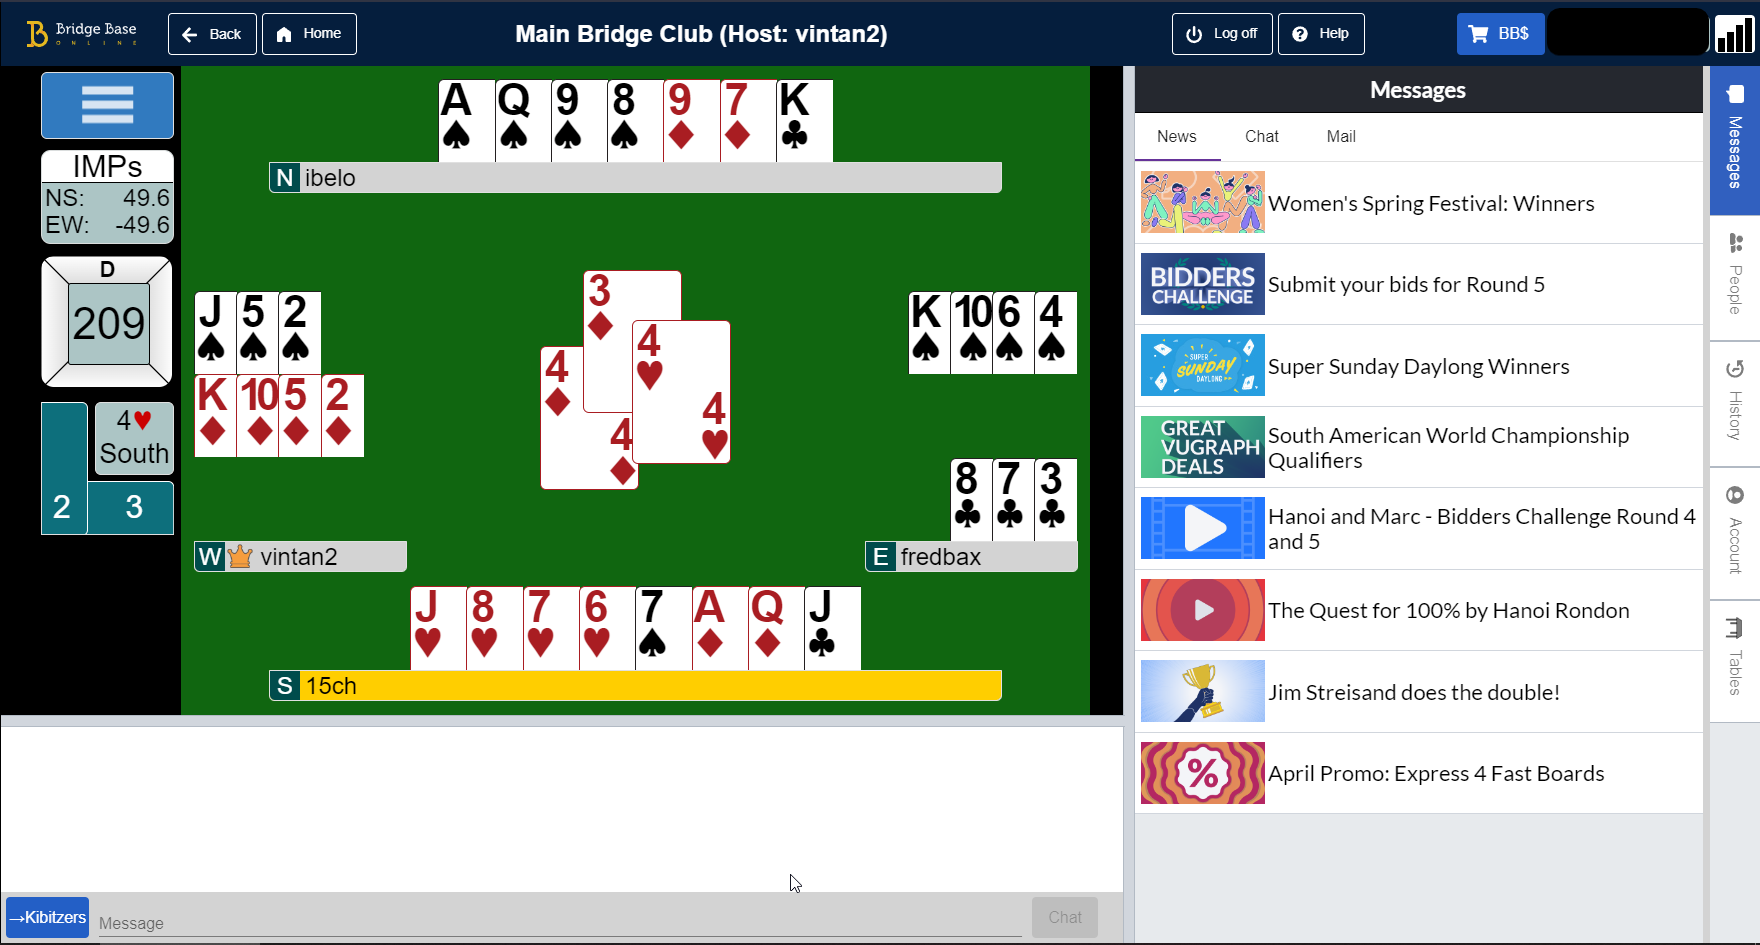
\includegraphics[width=\textwidth]{img/brydz-platformy/bridgebase.png}
  \caption{Rozgrywka brydża na platformie Bridge Base}
  \label{fig:bridge-base}
\end{figure}

\begin{figure}[h]
  \centering
  \hfill
  \subfloat[Główny ekran rozgrywki]{
    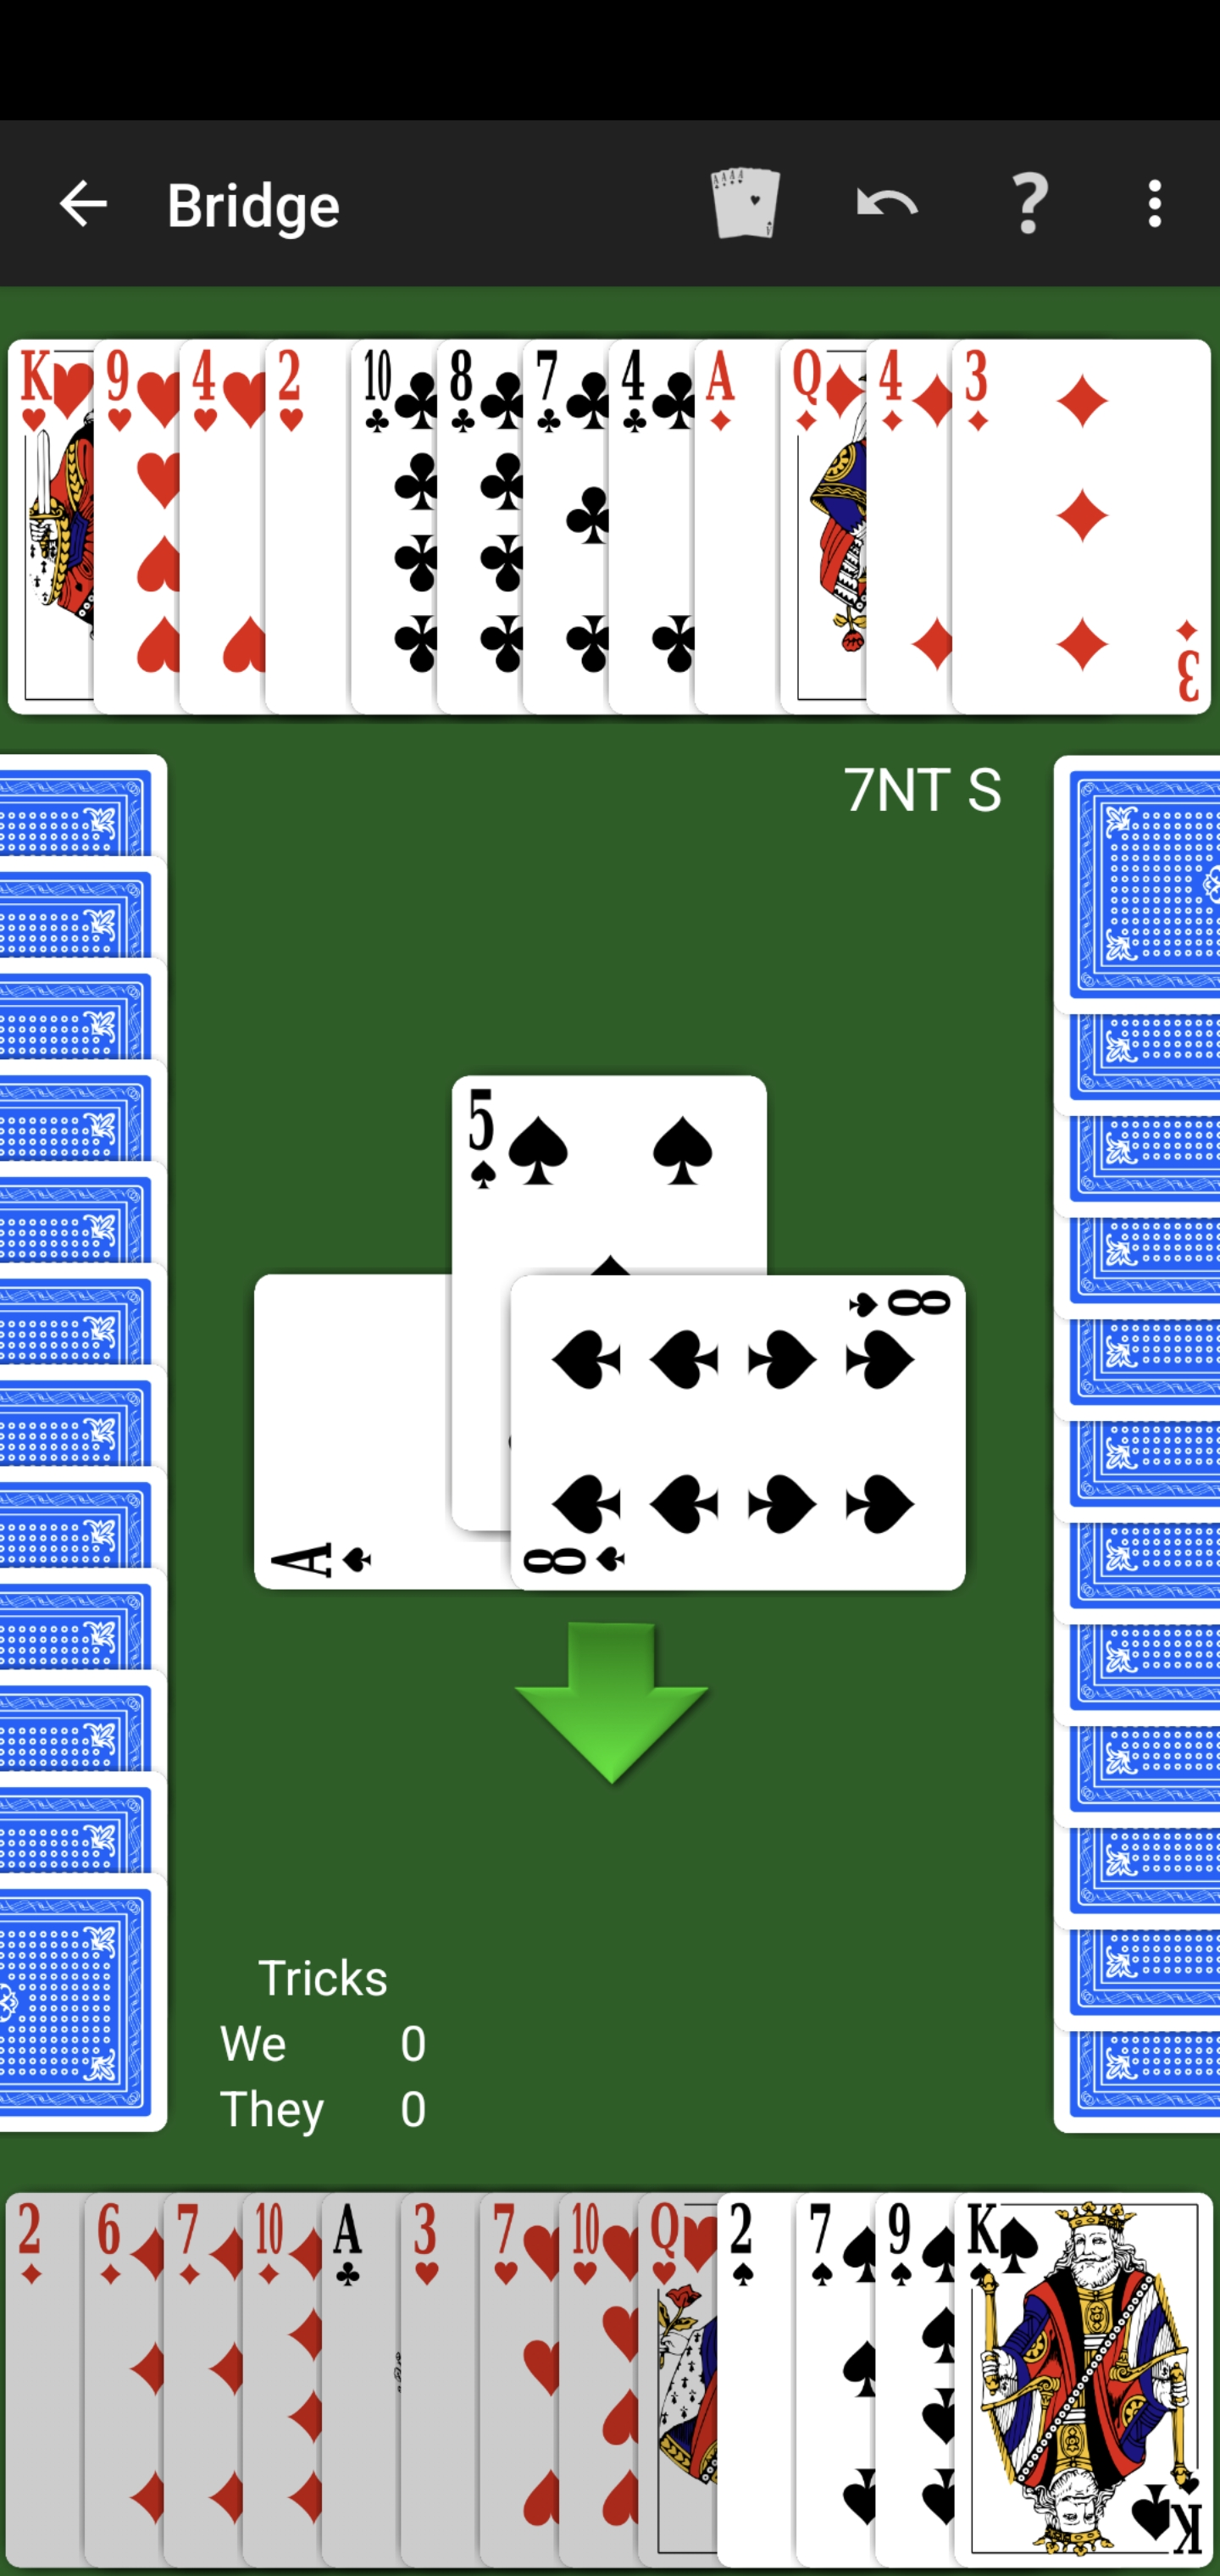
\includegraphics[width=.4\textwidth]{img/brydz-platformy/neuralplay1.jpg}
    \label{fig:neural-play-1}
  }%
  \hfill
  \subfloat[Historia bieżącej rozgrywki]{
    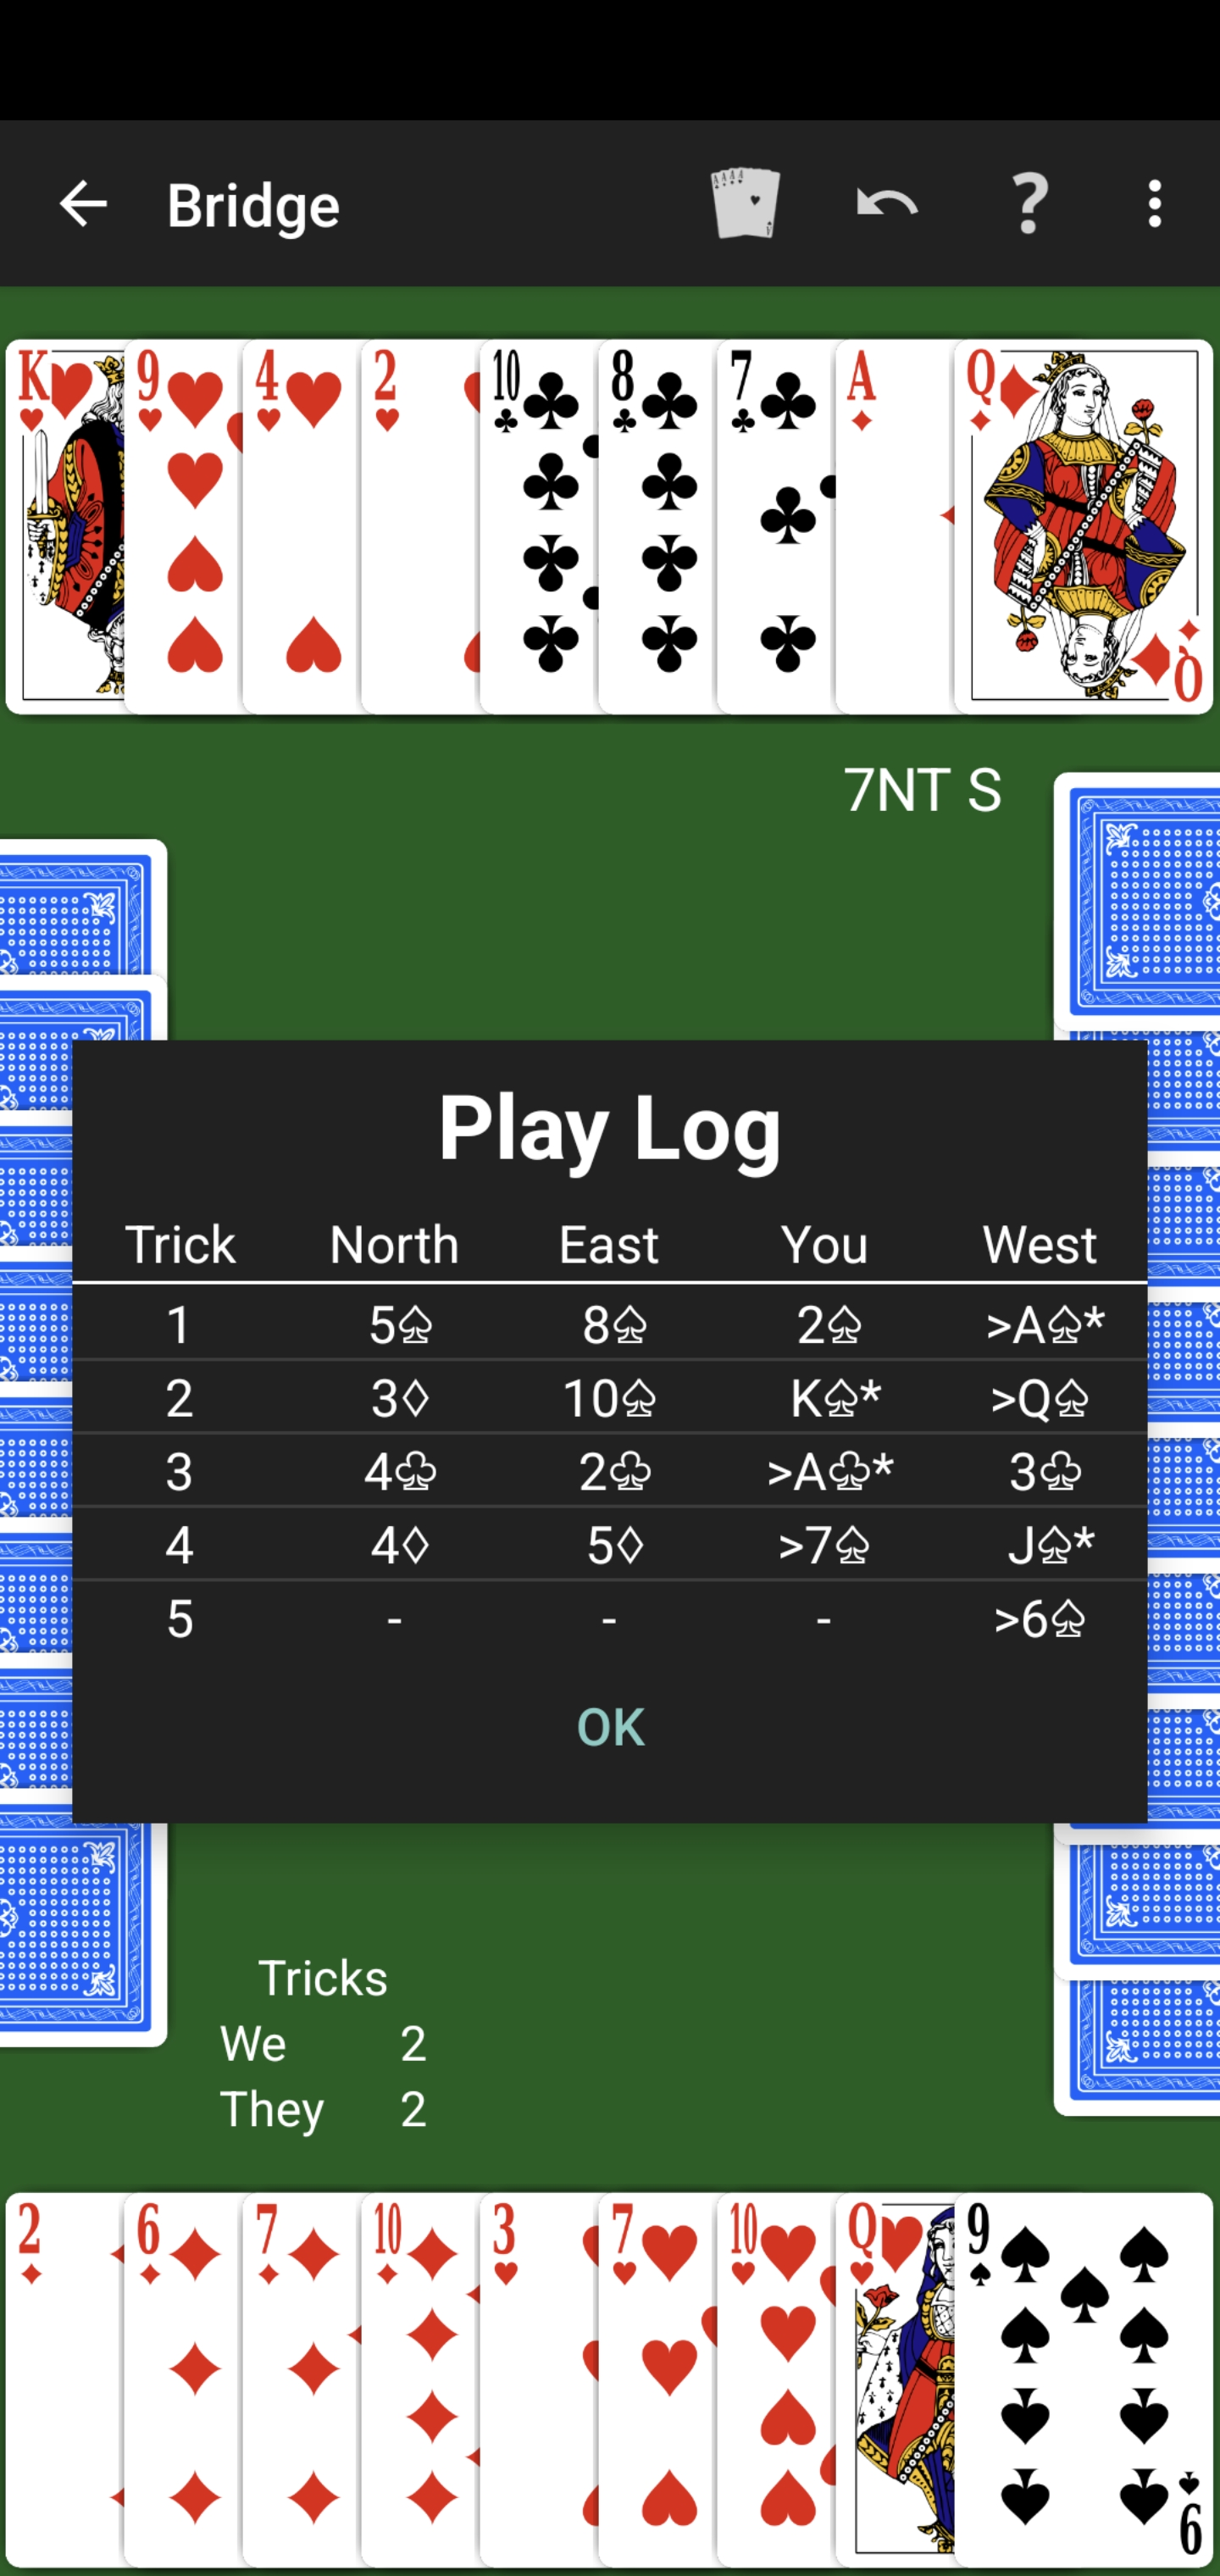
\includegraphics[width=.4\textwidth]{img/brydz-platformy/neuralplay2.jpg}
    \label{fig:neural-play-2}
  }%
  \hfill
  \caption{Rozgrywka brydża w aplikacji Bridge by NeuralPlay}
  \label{fig:neural-play}
\end{figure}
\FloatBarrier

\section{Wizja produktu}

Produktem będzie aplikacja webowa (desktopowa) umożliwiająca grę w~brydża,
bez konieczności posiadania partnera do gry. Realnego gracza w~rozgrywce
będzie mógł zastąpić Asystent AI. Jego zadaniem jest zapewnienie odpowiedniego
partnera lub przeciwnika dla graczy. Dodatkowo, w~trybie nauki, Asystent będzie pełnił rolę nauczyciela,
który może pomóc poprawić umiejętności graczy. Oprócz samego udziału
asystenta jako pomoc w~rozgrywce, będzie także oferować analizę historycznych
rozgrywek. Pomoże to graczom w~lepszym zrozumieniu gry i~dostarczeniu im
wskazówek dotyczących strategii.

Aplikacja będzie umożliwiała grę w~brydża z~udziałem jednego lub więcej graczy,
którzy będą mogli połączyć się przez Internet, dzięki centralnemu serwerowi.
Zamierzamy zaprojektować ją w~taki sposób, aby była intuicyjna i~łatwa
w~obsłudze dla wszystkich użytkowników, zarówno początkujących, jak
i~doświadczonych graczy.

%%%

\section{Stos technologiczny}

Aplikacja internetowa zostanie napisana w~frameworku React \cite{React}.
Zdecydowaliśmy się na ten wybór, ze względu na dużą popularność tej
technologii. W~2022 roku serwis Stack Overflow \cite{StackOverflow} przeprowadził ankietę dotyczącą między innymi wykorzystywanych technologii
webowych \cite{React-stack}. Aż 42.62\% respondentów wybrało React,
zajmując 2 miejsce w~rankingu. Jako, że wykorzystuje on język Javascript,
który według wspomnianej ankiety jest najpopularniejszym językiem programowania,
dostępna jest olbrzymia baza bibliotek i~sprawdzonych rozwiązań. Za wizualną
część projektu będzie odpowiedzialny framework Tailwind CSS \cite{Tailwind}.
Oferuje on gotowe klasy CSS, które pozwalają na szybkie tworzenie responsywnych
i~estetycznych interfejsów. Część serwerowa obsługująca sesje gier zostanie
napisana w~języku Python \cite{Python} za pomocą biblioteki FastAPI
\cite{FastAPI}. Funkcjonalność związana z~obsługą użytkowników i~gromadzenia
danych będzie wykorzystywała usługę Google Firebase \cite{Firebase}.

Asystent AI zostanie zrealizowany jako osobny program serwerowy
udostępniający własne API. Backend obsługujący sesje gier
będzie mógł wysłać do API Asystenta aktualny stan gry, aby otrzymać
odpowiedź zawierającą analizę tego stanu, między innymi
prawdopodobieństwo wygrania każdej z~par graczy oraz listę
najlepszych ruchów, jakie mogą być wykonane przez następnego gracza.

Została przewidziana możliwość zastosowania wielu algorytmów AI
do brydża. W~kolejności od najbardziej ambitnego do
najprostszego w implementacji, są to:
\begin{enumerate}
  \item algorytm Regularized Nash Dynamics \cite{doi:10.1126/science.add4679},
  \item algorytm AlphaZero \cite{Silver2017MasteringCA} połączony
        z algorytmem IS-MCTS \cite{6203567},
  \item implementacja algorytmu IS-MCTS z biblioteki OpenSpiel \cite{LanctotEtAl2019OpenSpiel},
  \item program AI do brydża GIB \cite{Ginsberg1999GIBST},
  \item algorytm Pure Monte Carlo Tree Search \cite{pmcts},
  \item algorytm ,,random move''.
\end{enumerate}

Opcja 1. dotyczy implementacji algorytmu przedstawionego w~artykule
\cite{doi:10.1126/science.add4679}.
Opcja 2. to autorski pomysł rozwinięcia algorytmu IS-MCTS.
Ideą jest użycie transformacyjnej sieci neuronowej do predykcji
determinizacji stanu gry, która jest potrzebna w~algorytmie IS-MCTS.
Następnie, algorytm AlphaZero zostałby zastosowany do przeszukiwania
drzewa zbiorów informacji tworzonego przez IS-MCTS.
Pozostałe opcje polegają na zastosowaniu gotowych rozwiązań lub
prymitywnych algorytmów.

%%%

\section{Analiza zagrożeń}

Gra w~brydża jest jedną z~najtrudniejszych gier strategicznych na świecie.
Do tej pory nie powstał żaden system AI grający na mistrzowskim poziomie
uwzględniający pełną wersję gry z~licytacją \cite{Bethe2021AdvancesIC}.
Stworzenie gracza AI o~wystarczająco wysokim poziomie umiejętności może być
trudne. W~literaturze zostało opisane wiele metod AI do brydża
\cite{Zhang2019DesignAD,Zhang2022TheSO,Zhang2022AIEB,Ginsberg1999GIBST}
co sugeruje, że jest to temat dalej otwarty i~ciągle rozwijany.
Przedstawiliśmy 6 różnych możliwości implementacji AI.
W~razie problemów z~implementacją jednej z~nich, pozostałe
zostaną wykorzystane jako plany awaryjne.

Ważnym elementem każdej gry online jest niezawodność systemu
backend oraz jego odporność na awarie.
Aplikacja musi być również odporna na problemy sieciowe.
Platforma Firebase zapewnia nam mechanizmy zabezpieczające
przed problemami po stronie klienta, połączenia internetowego
oraz samego backendu Firebase, który jest redundantnie
rozproszony po całym świecie.
Samo hostowanie strony internetowej zostanie zrealizowane
usługą Firebase Hosting, która również zapewnia wysoką
niezawodność.
Bezpieczeństwo aplikacji będzie zarządzane za pomocą
usługi Firebase Authentication.

Powyżej wymienione usługi są dostępne w darmowym planie.
Podczas pracy nad projektem może dojść do sytuacji, że
zostaną one przekształcone w~plan płatny.
Jeśli dostępne platformy chmurowe staną się niedostępne,
zastosowany zostanie własny serwer działający
w~oparciu o~komputer osobisty lub mikrokomputer, np. Raspberry Pi \cite{RPi}.

%%%

\section{Szkic aplikacji}

% \begin{figure}[h]
%   \centering
%   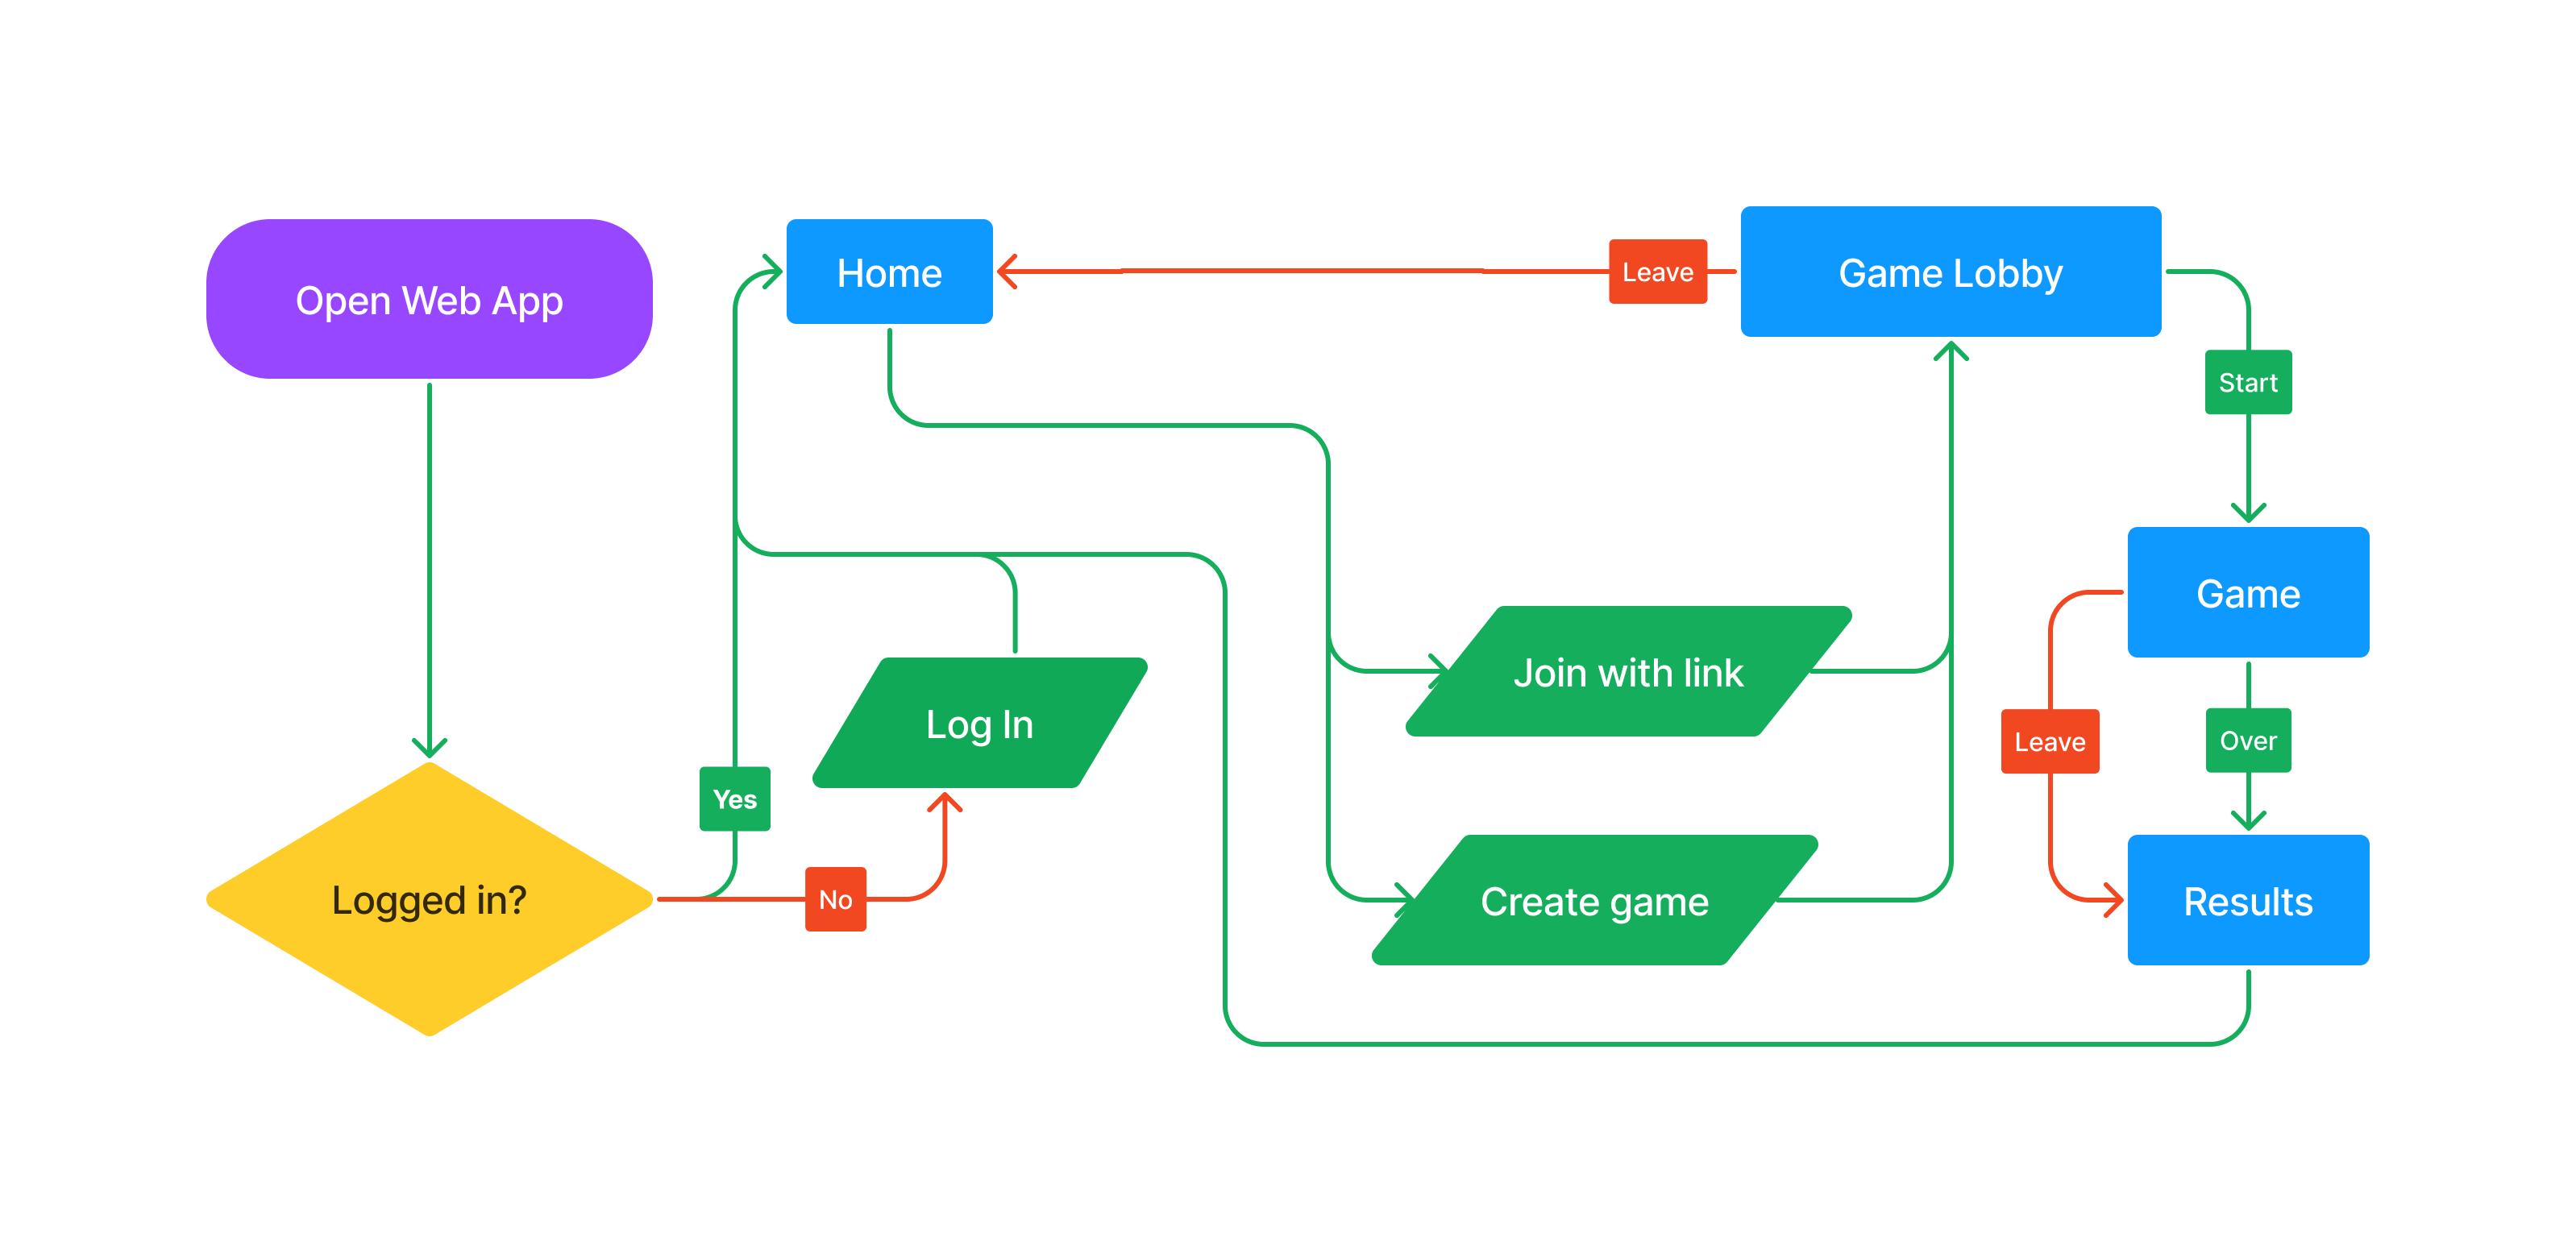
\includegraphics[width=\textwidth]{img/user_flow.png}
%   \caption{Schemat interakcji z aplikacją}
% \end{figure}

\begin{figure}[h]
  \centering
  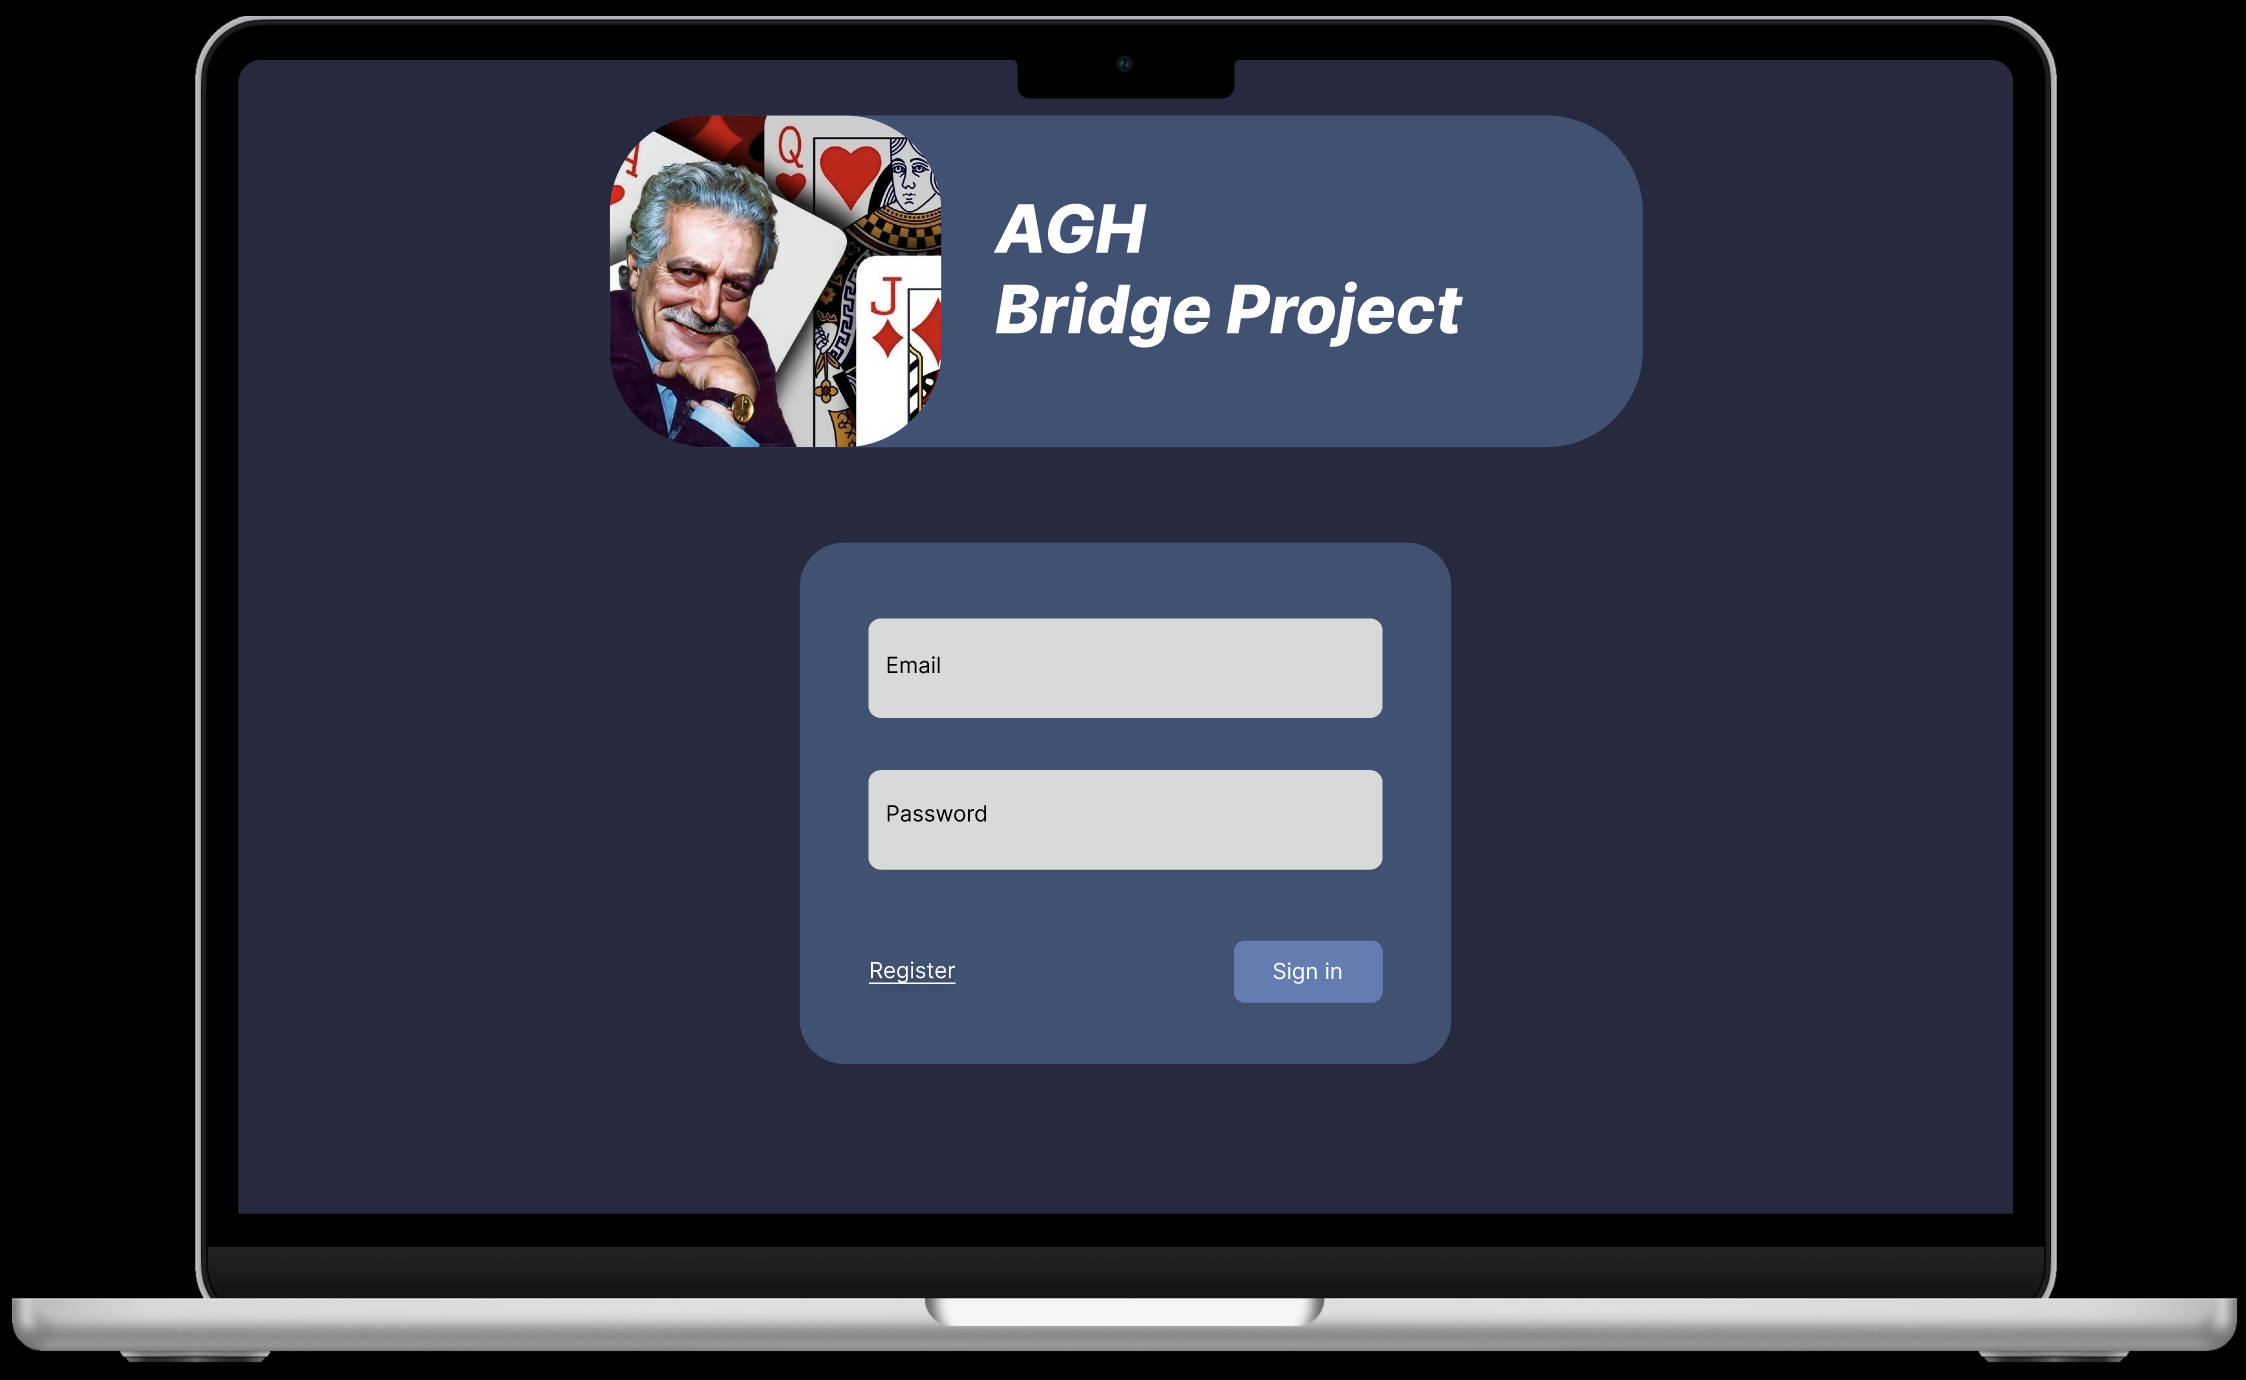
\includegraphics[width=\textwidth]{img/figma-szkic/1.png}
  \caption{Ekran logowania}
\end{figure}

\begin{figure}[h]
  \centering
  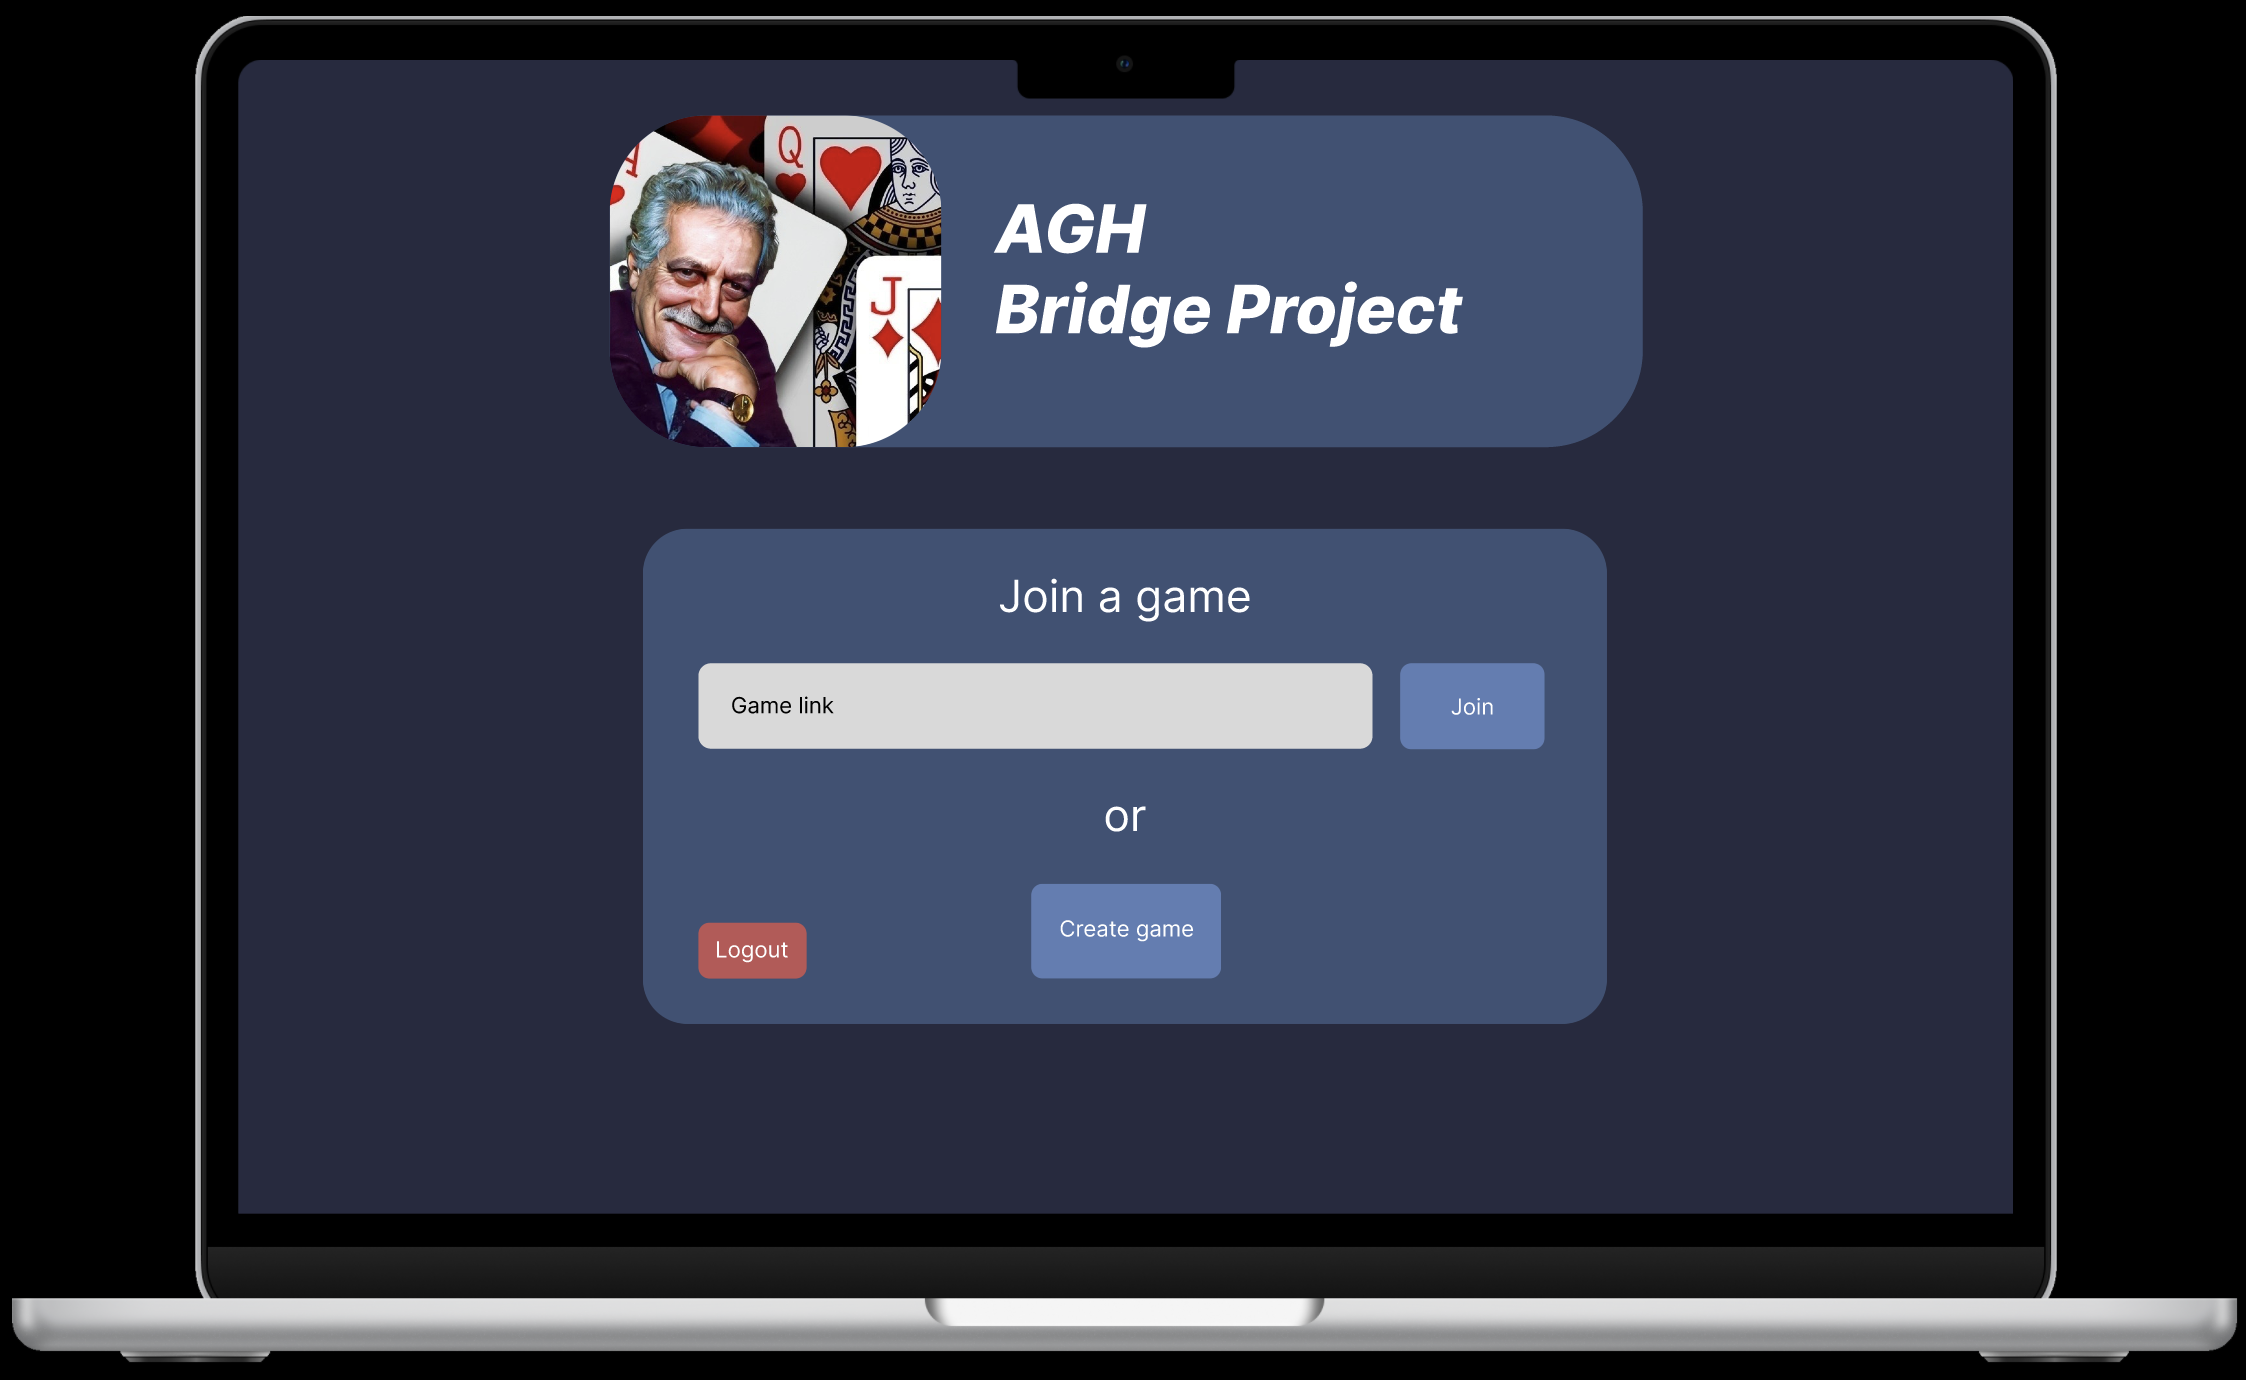
\includegraphics[width=\textwidth]{img/figma-szkic/2.png}
  \caption{Ekran główny}
\end{figure}

\begin{figure}[h]
  \centering
  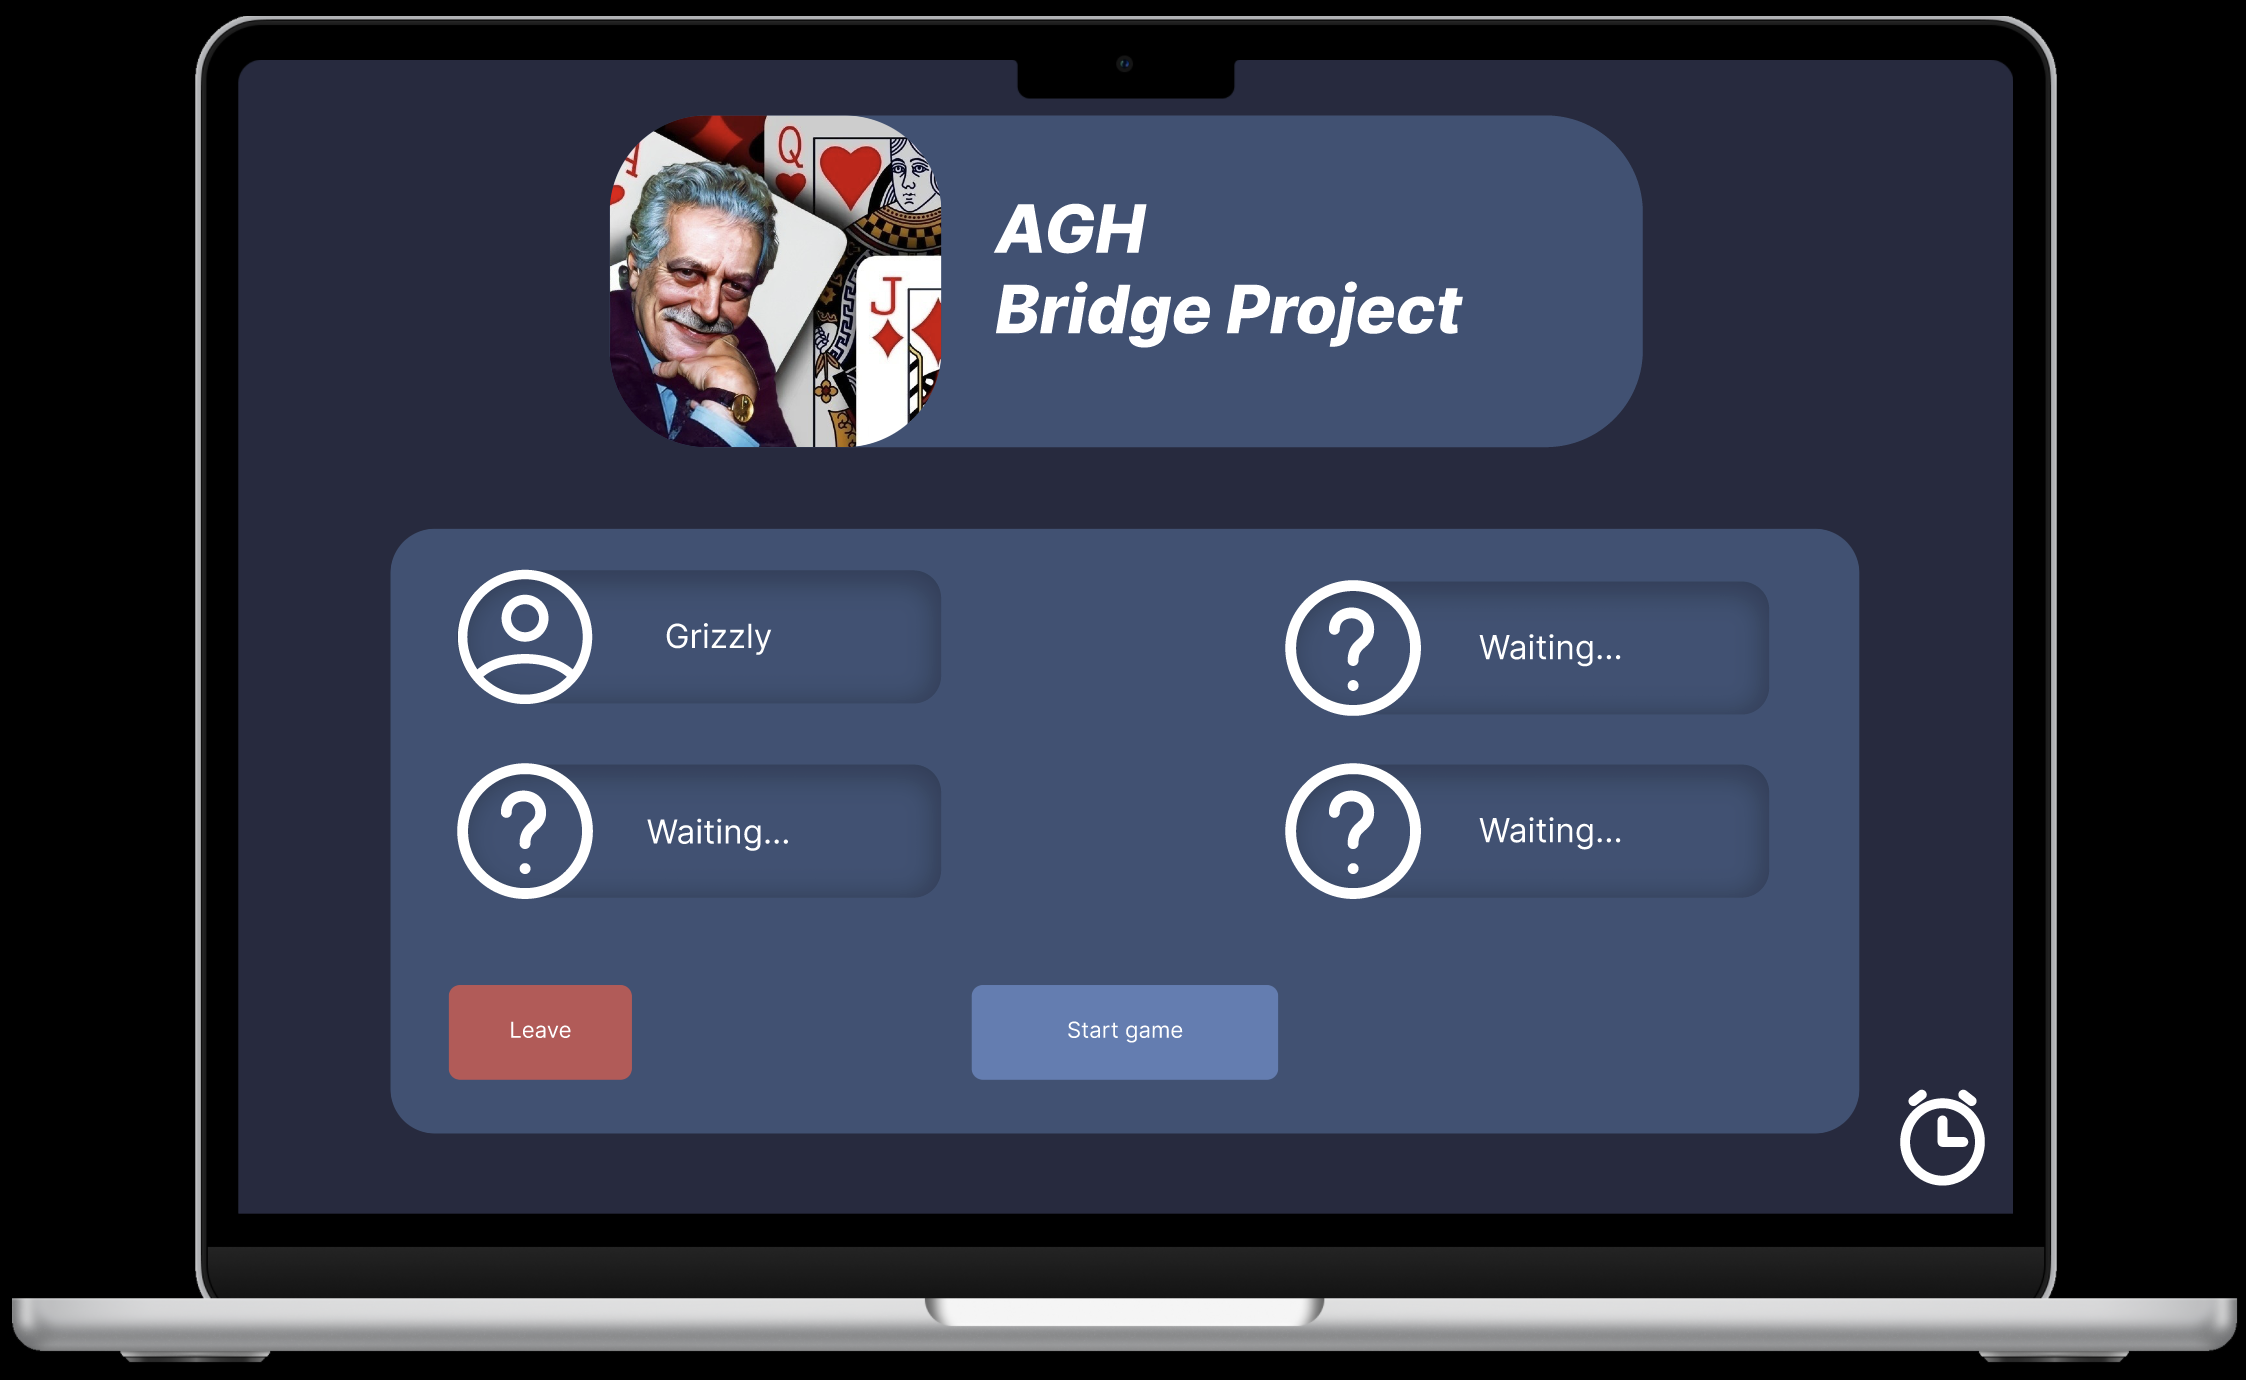
\includegraphics[width=\textwidth]{img/figma-szkic/3.png}
  \caption{Ekran lobby}
\end{figure}

\begin{figure}[h]
  \centering
  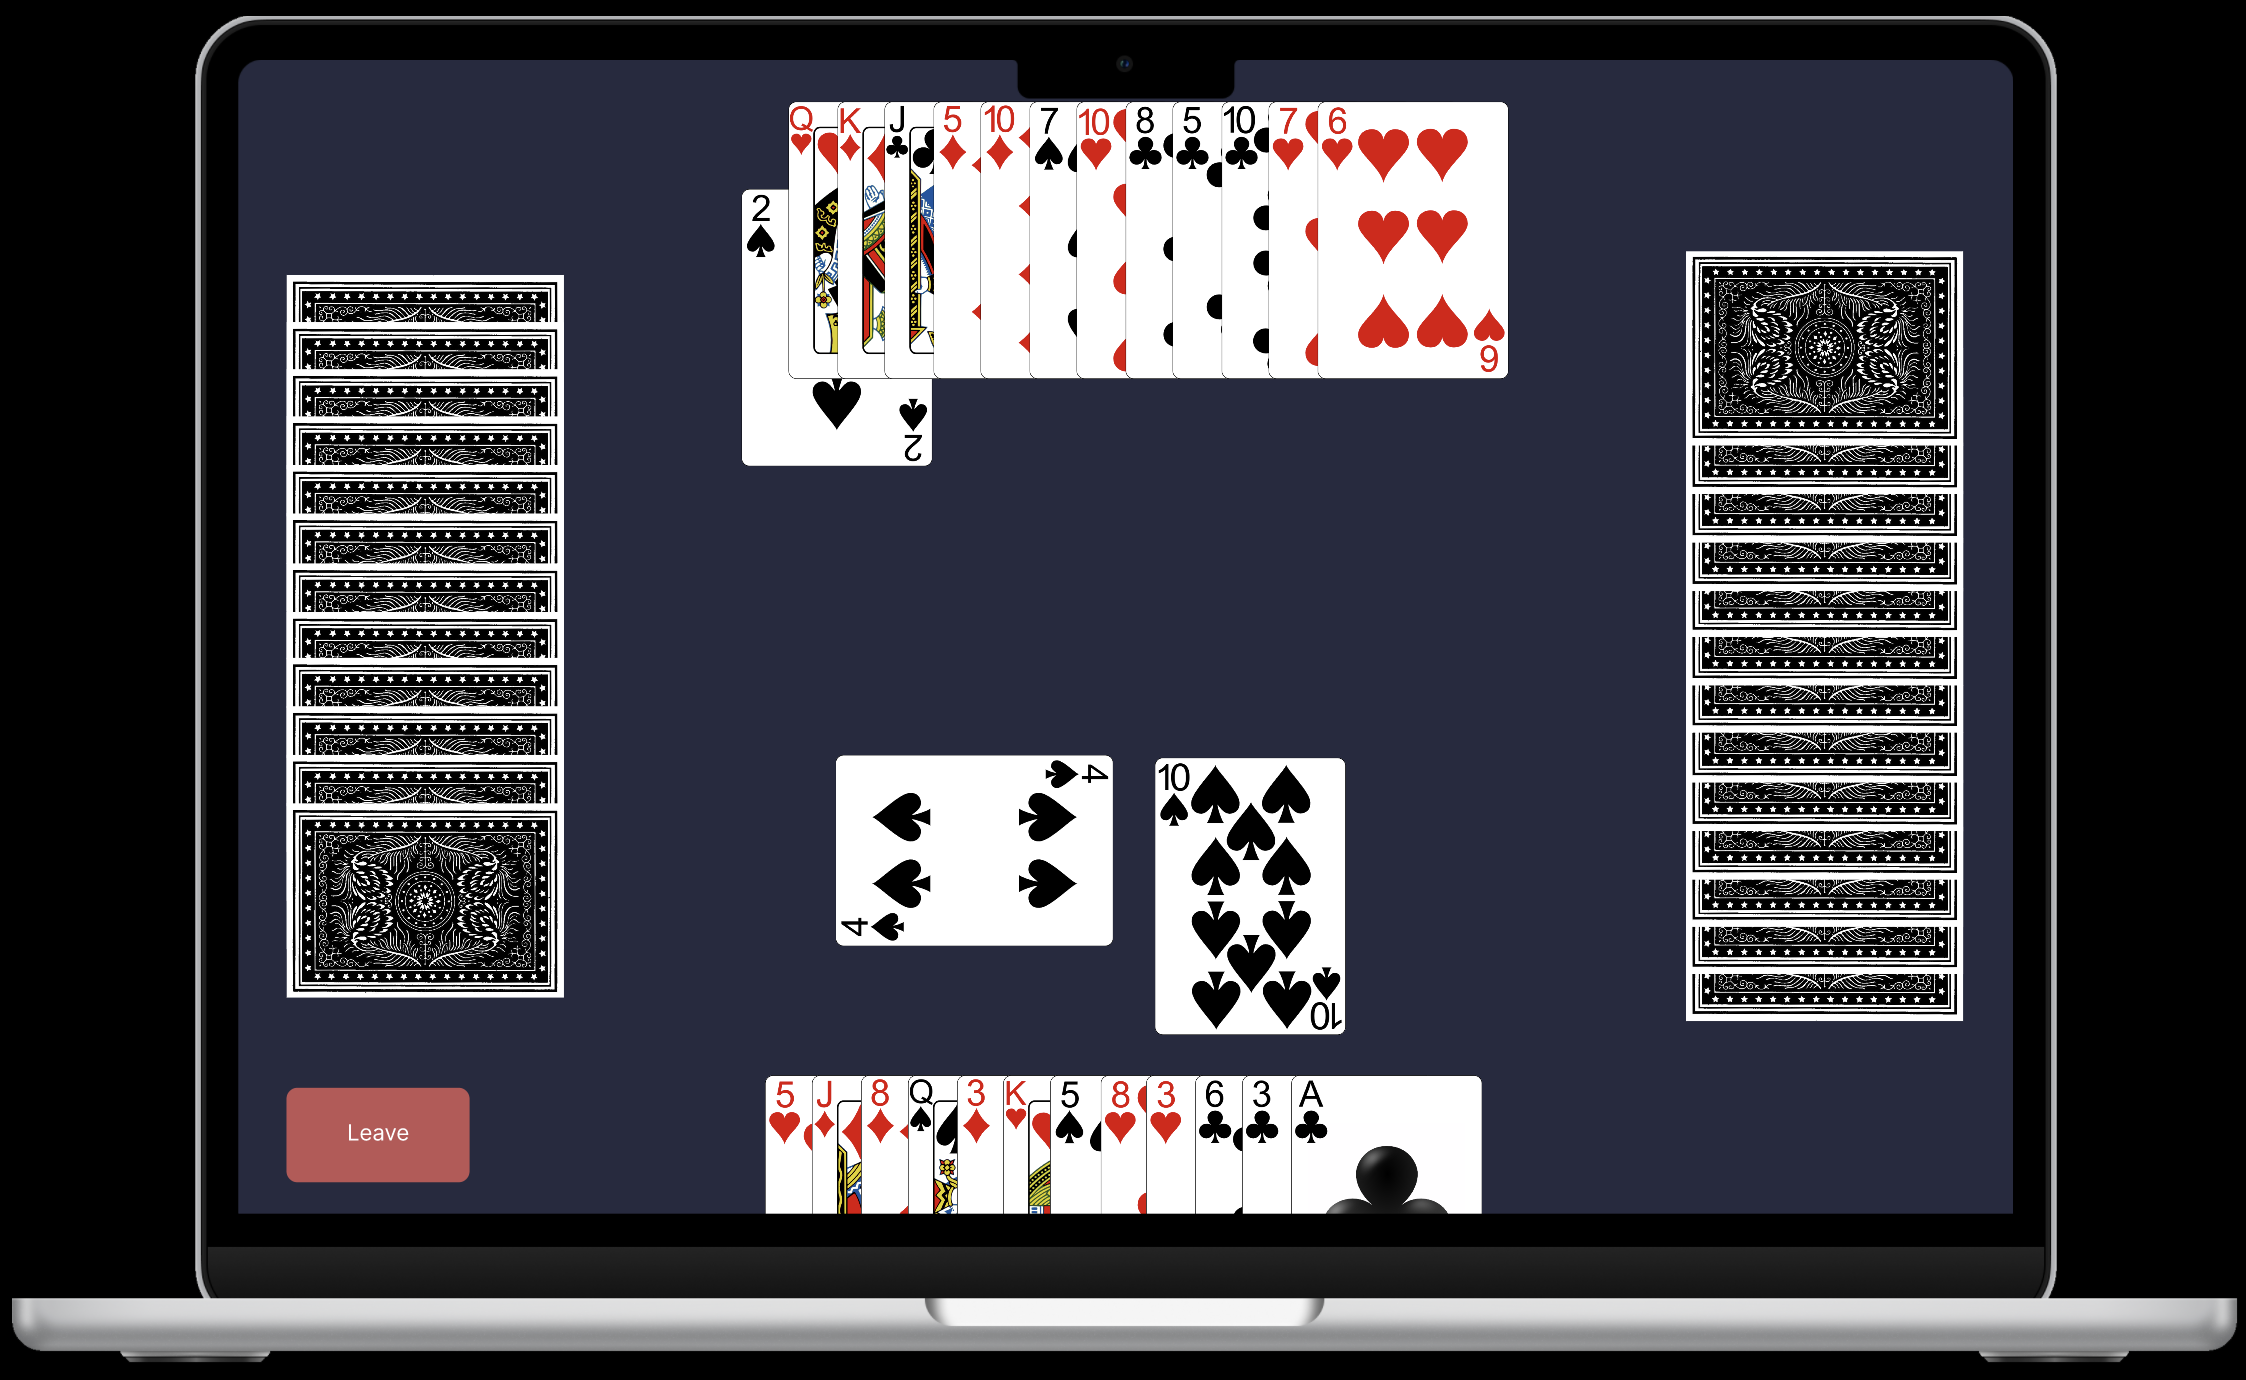
\includegraphics[width=\textwidth]{img/figma-szkic/4.png}
  \caption{Ekran gry}
\end{figure}

\FloatBarrier


\section{Słownik pojęć}

\begin{enumerate}
  \item Brydż - karciana gra strategiczna rozgrywana przez dwie pary graczy,
  \item Użytkownik - człowiek grający w brydża za pomocą aplikacji,
  \item Gracz - człowiek lub program grający w brydża,
  \item Partner - drugi gracz grający w parze danego gracza,
  \item Przeciwnik - jeden z graczy z pary grającej przeciwko danemu graczowi,
  \item Asystent AI - program posiadający możliwość analizy rozgrywki w celu nauki, współpracy lub konkurencji z użytkownikiem,
  \item Wirtualny Partner - partner symulowany przez Asystenta AI,
  \item Wirtualny Przeciwnik - przeciwnik symulowany przez Asystenta AI,
\end{enumerate}